%!TEX root = ../thesis.tex
%*******************************************************************************
%****************************** Fourth Chapter *********************************
%*******************************************************************************

\chapter{Benchmark}
\label{chap:benchmark}
\ifpdf
    \graphicspath{{Chapter4/Figs/Raster/}{Chapter4/Figs/PDF/}{Chapter4/Figs/}}
\else
    \graphicspath{{Chapter4/Figs/Vector/}{Chapter4/Figs/}}
\fi

\topic{Il faut un benchmark solide pour comparer les méthodes}

\section{Constitution du benchmark} % (fold)
\label{sec:constitution_du_benchmark}

\content{Weak baselines, too many (too complex or specific) objective functions and other problems in presenting ML results.}

\victor{Ce que j'essaie de faire c'est mettre un peu d'ordre. Donc je doit décrire les métriques utilisée par les autres papier. Décrire ce que je veux ranger}




\section{Higgs data} % (fold)
\label{sec:higgs_data}




\subsection{Simulation} % (fold)
\label{sub:simulation}

Precise simulation is not only used for training machine learning models.
Simulation is critical for the design of the apparatus itself or planning an upgrade of the apparatus.
Simulation allows to predict how the data should be according to a given version of the standard model.
Theorists updates on the standard model can be validated or rejected efficiently by comparing their predictions through simulation to the data.

Of course simulation of an experiment at the LHC requires tremedous work.
For example the ATLAS simulation \cite{Aad_2010} can be broken down into 3 major steps.
First the event simulation that takes care of the collision, the particles creation, the particle interactions between themselves and their decay to other particles.
Second the interaction between the particles and matter (the apparatus) which is done using Geant4 \cite{AGOSTINELLI2003250}, \cite{1610988}, \cite{ALLISON2016186}.
This is the part I find the most impressive.
Sensors, magnetic field generated by the electronics, cables, even the air or the cooling liquids are taken into account.
Finally digitization deals with what numbers will come out of the previous interaction to be finally stored for later analysis.
Although very accurate simulations of all parts and phenomena is technically possible the computation power often limits its usage to more approximative ones. 
This leads to creating a custom tradeoff for each analysis to focus computation on the most relevant parts.

Interaction between particles and the sensors are again fundamentally stochastic.
A very large number of sensors is required to reach a high enough resolution to make accurate measurements.
As a consequence each sensor interaction with a particle creates a latent variable in the modeling of a single event.
Therefore 100 000 detector pieces lead to 100 000 latent variables making the marginal likelihood intractable (see \autoref{sub:inverse_problem}).

Simulation is expensive and possible processes include very rare events like Higgs boson creation.
Without \emph{importance sampling}\needcite it would be impossible to simulate enough events to get a representative sample of those rare processes.
Simulation runs independently for every processes.
Then the data are gathered with importance weights reprensenting their relative probability of occurrence.





\subsection{HiggsML challenge} % (fold)
\label{sub:higgsml_challenge}


The data were initially produced for the HiggsML challenge \cite{Adam-Bourdarios2014}.
It was a the most successfull challenge of its time with (some number of teams and submissions).
The data is now publicly available \needcite.
\victor{TODO : citer les autres articles qui ont utilisés HiggsML}

The HiggsML dataset is composed of 818238 events described by 17 primary features and 13 features derived from the primaries.
Near the end of the challenge X more constructed features known as "cooked features" became popular \needcite.
The cooked features help getting good classification perfomances\needcite in some context (what context ?).
The label designing if the event is a signal ($H\to \tau \tau$) or a backgroud (any other process) is of course available in the dataset as well.

Sample weights used for the kaggle challenge is not the same ... why again ?




\subsection{Fast re-simulator} % (fold)
\label{sub:fast_re_simulator}


In order to ease experiments, the first part of this work is to build a fast re-simulator of the events.
Indeed one event require on min of CPU time to be generated.
Regenerating the entire dataset for all the set of parameters values we might want to try would be too expensive.
However the parameters considered in this work only affect some of the final parts of the simulation and can be computed a posteriori.

A small library was published\needcite and a more recent version is available here\needcite.
This rest of this section will briefly explain how the event are re-generated for a different set of parameters.

The parameter of interest $\mu$ is the deviation of the expected number of signal from the predictions of the standard model.
Recomputing the data only requires to multiply the sample weights of the signal events with $\mu$.
This is already enough to build a complete workflow of the inference without nuisance parameter.

5 nuisance parameters are considered : tau energy scale, lepton energy scale, jet energy scale, soft term, nasty backgrounds.

\subsubsection{Energy scales} % (fold)
\label{ssub:energy_scales}

The tau energy scale is comming from apparatus imperfections leading to a slightly wrong scale of the measured energy of tau particle.
The lepton and jet energy scale are exactly analogus but with lepton particle and jets.
The 3 energy scales are independant from each other leading to 3 nuisance parameters $\alpha_{tes}, \alpha_{les}, \alpha_{jes}$. 
This nuisance parameter is basically a proportional factor on one or several primary features (eg. PRI\_tau\_pt) stained with non negligeable uncertainty.
Recomputing the events for a different value of the energy scale requires not only to multiply the primary features with the updated value but also all the features derived from this primaries.

\subsubsection{Soft term} % (fold)
\label{ssub:soft_term}

The missing energy transverse (met) is perturbated by a random vector sampled from a normal distribution which standard deviation is our nuisance parameter $\alpha_{st}$.
This is a more difficult systematic effect to infer from the data.
Just like the parameter of interest it isby definition impossible to infer the soft term from one example.


\subsubsection{Nasty background} % (fold)
\label{ssub:nasty_background}

The background distribution is a mixture of several processes.
The mixture coefficient of one of these processes is not known with enough precision.
\victor{c'est celui avec un detailLabel = W}
This nuisance parameter $\alpha_{nb}$ only requires to recompute the weights.
Since the parameter of interest is also linked with the sample weights, ie the amount of events, this nuisance parameter directly leads to an increase of the variance of our estimator $\hmu$.
Indeed a larger number of events in a bin can now be explained by an increase of $\mu$ or an increase of $\alpha_{nb}$.



\subsubsection{Mass MMC} % (fold)
\label{ssub:mass_mmc}

Unfortunately the MMC mass (what the hell is it ?) cannot be easilly recomputed from primaries.
Computing the MMC mass involves an expensive optimization step \victor{More details ?}.
Although DER\_Mass\_MMC is the a relevant feature (\textbf{see missing figure}) for classification it is removed from the dataset.

\victor{TODO : figure top 5 or top 10 feature importances}




\subsubsection{Bootstraping} % (fold)
\label{ssub:boostraping}


Re-generating the data is not the same as re-running the simulation.
\victor{Results on boostrapping that says when it is OK to do it ?}

Training the direct regression method requires way more data than training a classifier since a sample for a regressor is composed of thousands of events.
With boostrapping and considering the re-generation as data augmentation the finite HiggsML dataset can be turned into an almost infinite generator of events.




\section{Toy datasets} % (fold)
\label{sec:toy_datasets}


Toy datasets allow a full control of the generative process and the properties of the data.
It is a necessary step to produce a test bed of the program code.
But also to evaluate the influence of many parameter (eg. number of dimension, number of sample, signal/background separability, etc) on the performances to help explain the performances on real data.






\subsection{Toy 1D} % (fold)
\label{sub:toy_1d}

The first toy is a very simple case of estimation of a mixture coefficient in the presence of one systematic effect.
The likelihood is known and tracktable making maximum likelihood and bayesian inference possible.
Comparing the inference methods to the best possible inference is a first step to validate them.


The toy generative process is a mixture of 2 distributions with one observable $x \in \RR$.
The background distribution is a gamma distribution versus a gaussian distribution for the signal process.
\autoref{fig:minitoy_distrib} presents the data distribution.
To make the problem non trivial and correspond more to reality the signal distribution is overlapping with the background distribution.

The parameter of interest is the mixing coefficient $\mu$ of the 2 distributions.
The nuisance parameter $\alpha$ is a rescaling of the observable $x$.

Without nuisance parameter $\alpha$ the likelihood is :
$$
    p(x | \mu) = \mu \mathcal N(x|a, d) + (1-\mu) \Gamma(x|k, l)
$$

with $N(x|a, d)$ a gaussian with mean $a$ and standard deviation $d$ and $\Gamma(x|k, l)$ a gamma distribution with $k$ ... and $l$ the localization  ... ????
The chosen values are : $a = 5, d=0.5, k=2, l=0$.


Including nuisance parameter $\alpha$ the likelihood becomes :
$$
    p(x | \mu, \alpha) = \mu \mathcal N(x|\alpha a, \alpha d) + (1-\mu) \Gamma(x|\alpha k, l)
$$

\begin{figure}[htb]
    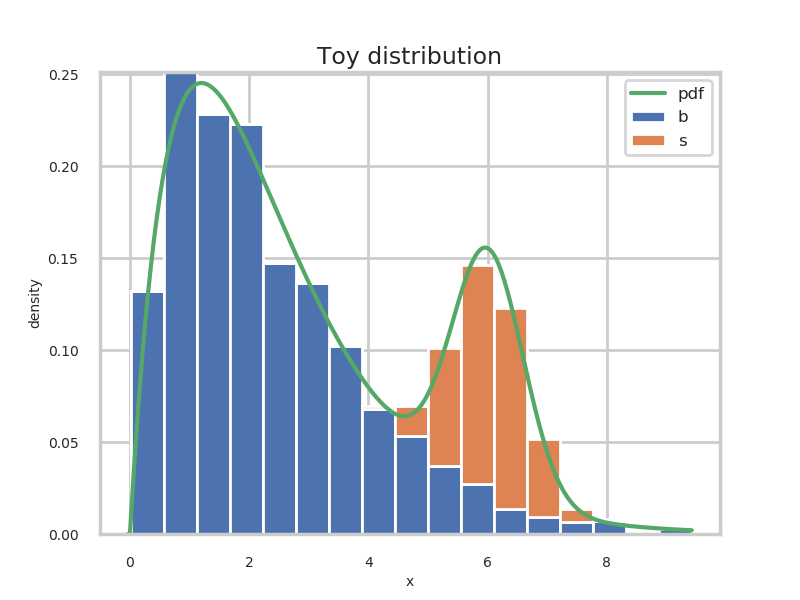
\includegraphics[width=\linewidth]{minitoy/distrib.png}
    \caption{Data distribution of the 1D toy for a 10,000 instances sampling}
    \label{fig:minitoy_distrib}
\end{figure}






\subsection{Toy 3D} % (fold)
\label{sub:toy_3d}

To get closer to reality the toy example introduced in \cite{DECASTRO2019170inferno} is also included.
It is a mixture of 2 processes : $f_b$ for the backgrounds and $f_s$ for the signals.

\begin{equation}
	f_b (x|r, \lambda) = \mathcal N \left ( (x_0, x_1) | (2+r, 0) 
	\begin{bmatrix} 5 & 0 \\ 0 & 9 \end{bmatrix} \right ) Exp((x_2| \lambda)
\end{equation}
\begin{equation}
	f_s (x|r, \lambda) = \mathcal N \left ( (x_0, x_1) | (1, 1) 
	\begin{bmatrix} 1 & 0 \\ 0 & 1 \end{bmatrix} \right ) Exp((x_2| 2)
\end{equation}

Leading to the likelihood :
\begin{equation}
	p(x | r, \lambda, \mu ) = (1-\mu) f_b(x|r, \lambda) + \mu f_s(x|r, \lambda)
\end{equation}

This toy is multi dimensional, more complex and includes 2 nuisance parameters.
The nuisance parameters affects only the background distribution.
Once again the background and signal distribution are overlapping.
\autoref{fig:s3d2_pairgrid} shows the distributions of a sampled dataset.

\begin{figure}[htb]
    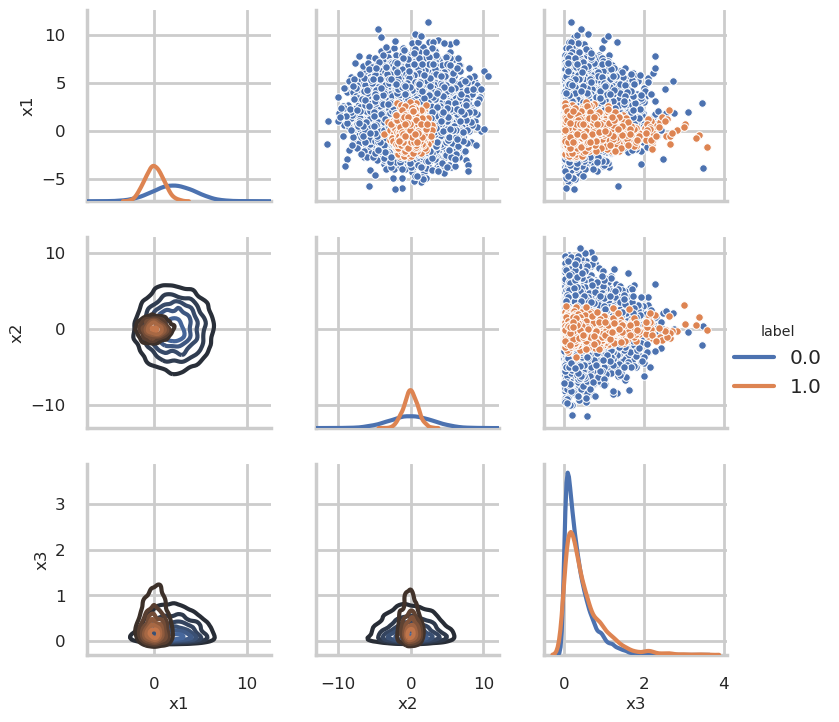
\includegraphics[width=\linewidth]{s3d2/pairgrid}
    \caption{Data distribution of the 3D toy}
    \label{fig:s3d2_pairgrid}
\end{figure}






\section{Bayesian inference on toys} % (fold)
\label{sec:bayesian_inference_on_toys}


The toy problems (see \autoref{sub:toy_1d} and \autoref{sub:toy_3d} ) do not suffer from intractable likelihood making it possible to compute the posterior probability using standard bayesian inference.
The computed posterior is the best possible inference and will be compared with the other methods that assumes the samplewise likelihood is intractable.

\subsection{Computing the posterior} % (fold)
\label{sub:computing_the_posterior}

The marginal posterior probability density function of the parameter of interest $p(\mu|D)$ can be computed from the likelihood and a prior.
The prior is chosen as uniform over the domain of possible values of the parameters $\mu$ and $\alpha$.
A dataset $D$ of independant and identically distributed samples is assumed to be available.

From Bayes theorem : 
\begin{equation}
    p(\mu, \alpha | D) = \frac{p(D|\mu, \alpha) p(\mu, \alpha)}{p(D)} = \frac{p(D|\mu, \alpha) p(\mu, \alpha)}{\int_{\alpha, \mu} p(D|\alpha, \mu) p(\mu, \alpha) d\alpha d\mu}
\end{equation}
and
\begin{equation}
	p(\mu|D) = \int_{\alpha} p(\mu, \alpha | D) p(\alpha|D) d\alpha
\end{equation}

Computing the integrals by hand can be tedious.
The inference can be approximated with a fine discretization of the continuous space of parameter.
It starts with a grid $\{\mu_i, \alpha_j\}_{i,j}$, fine enough, covering the space of possible values of the parameters.

Then we can compute the likelihood
\begin{equation}
	p(D|\mu_i, \alpha_j) = \prod_{x_k\in D} p(x_k|\mu_i, \alpha_j)
\end{equation}
Dealing with products of probabilities leads to numerical instability.
The number of samples can easily be big enough to obtain numbers too small to be precisely stored in a 64 bits float.
The usual trick is to work with log probabilities which gives the following tensor 
\begin{equation}
	L_{ij} = \log (p(D|\mu_i, \alpha_j)) = \sum_{x_k\in D} \log (p(x_k|\mu_i, \alpha_j))
\end{equation}
Combining it with a prior tensor $K_{ij} = \log(p(\mu_i, \alpha_j))$ the tensor $ R_{ij} = \log(p(D|\mu_i, \alpha_j)) + \log(p(\mu_i, \alpha_j) )$ gives access to the posterior $p(\mu_i, \alpha_j | D)$ through renormalization with $p(D)$.
Recall that :
\begin{equation}
    p(D) = \int_{\alpha, \mu} p(D|\alpha, \mu) p(\mu, \alpha) d\alpha d\mu
\end{equation}
Which gives after discretization
\begin{equation}
    p(D) = \sum_{\alpha_j, \mu_i} p(D|\alpha_j, \mu_i) p(\mu_i, \alpha_j)
\end{equation}
\begin{equation}
	T_{ij} = p(\mu_i, \alpha_j | x) = softmax(R_{ij}) = \frac{ e^{ R_{ij} }  }{ \sum_{ij} e^{ R_{ij} } }
\end{equation}

The marginal probabilities are computed from $T_{ij}$ :
\begin{equation}
	p(\mu_i | D) = \sum_j T_{ij} = M_i
\end{equation}
\begin{equation}
  p(\alpha_j | D) = \sum_i T_{ij} = A_j
\end{equation}
The method presented here is quite simple but leads to very accurate estimation on the toy problems.


\subsection{Extract quantities from discretized marginal posterior} % (fold)
\label{sub:extract_quantities_from_discretized_marginal_posterior}

A plot of $p(\mu | D)$ is not the best way of comparing the bayesian inference to the other methods.

If the distribution $p(\mu | D)$ is well behaving the expectation of $\mu$ will be close to the maximum.
\begin{equation}
	\hat\mu = \EE[\mu|D] = \sum_i \mu_i M_i
\end{equation}
The confidence interval is then the variance
\begin{equation}
	\VV(\mu|D) = \sum_i \mu_i^2 M_i - (\sum_i \mu_i M_i)^2
\end{equation}

This variance can be splitted into two contribution : the statistical variance $\EE_{\alpha \sim p(\alpha|x)}[ \VV(\mu|x, \alpha) ]$ and the systematic variance $\EE_{\alpha \sim p(\alpha|D)} \left ((\EE [\mu|D, \alpha]  - \EE[\mu|D])^2\right )$

\begin{align}
	\EE_{\alpha \sim p(\alpha|D)}[ \VV(\mu|D, \alpha) ] 
			&= \sum_j \VV(\mu|D, \alpha_j) p(\alpha_j | x) \\
			&= \sum_j \VV_i(\mu_i, \frac{T_{ij}}{A_j}) A_j
\end{align}
\begin{align}
	\EE_{\alpha \sim p(\alpha|D)} \left ((\EE [\mu|D, \alpha]  - \EE[\mu|D])^2\right ) 
			&= \VV(\mu|D) - \EE_{\alpha \sim p(\alpha|D)}[ \VV(\mu|D, \alpha) ] \\
			&= \VV(\mu_i, M_i) - \sum_j \VV_i(\mu_i, T_{ij}) A_j
\end{align}

\subsubsection{Note 1}

The neural network regressor is learning to compute either $p(\mu_i |D, \alpha_j) = \frac{p(\mu_i, \alpha_j | D)}{p(\alpha_j | D)} = \frac{T_{ij}}{A_j} = N_{ij}$ or $p(p(\mu_i |D) = = \sum_j T_{ij} = M_i$
Meaning that it is possible to compare the MDN regressor output to the true distribution.


\subsubsection{Note 2}

If there is multiple nuisance parameters $\alpha$, $\beta$, etc the tensor are simply n-dimensional : $L_{ijk...}$, $T_{ijk...}$, $K_{ijk...}$, etc.
And all sums over $j$ become summs over $j,k, ...$ which is easy to handle with broadcasting in modern numeric libraries.



\section{Evaluation metric} % (fold)
\label{sec:evaluation_metric}

\topic{The evaluation metric is the empirical mean squared error on the estimated parameters including variances}

Many methods to estimate the parameter of interest and its variance are available.
If changing the set of hyper parameter for the learning procedure is considered as changing the method then countless methods are to be evaluated.
Automating the measure of the performances of a proposed method is crucial to select the best method.
In this section is described a simple but general procedure to measure the performances of a given method.

The usual criterions to evaluate an estimator $\htheta$ are the bias, the variance and the mean squared error defined as follow :
\begin{equation}
  Bias(\htheta) = \EE[\htheta] - \thetas
\end{equation}
\begin{equation}
  Var(\htheta) = \EE[ (\htheta - \EE[\htheta])^2 ] = \EE[\htheta^2] - (\EE[\htheta])^2
\end{equation}
\begin{equation}
  MSE(\htheta) = \EE[(\htheta - \thetas)^2] = Var(\htheta) + [Bias(\htheta)]^2
\end{equation}

To evaluate these criterion we need to repeat the experiement $N$ times leading to many estimation of the parameters $\hmu^{(k)}$ and $\hshmu^{(k)}$.
Repeating the experiment can be done through cross-validation methods.


\subsection{Evaluation of the parameter of interest estimator} % (fold)
\label{sub:evaluation_of_the_parameter_of_interest_estimator}

First, let's focus on evaluating the estimator of the parameter of insterest $\hmu$.
The true value of $\mu$, noted $\mus$, is available during tests since it is an input of the simulator.

From the estimation of its expected value
\begin{equation}
  \EE[\hmu] \approx <\hmu^{(k)}>_k = \frac{1}{N} \sum_{k} \hmu^{(k)}
\end{equation}
it is possible to estimated the criterions

\begin{equation}
  Bias(\hmu) \approx <\hmu^{(k)}>_k - \mus
\end{equation}
\begin{equation}
  \label{eq:var_hmu}
  Var(\hmu) \approx <\hmu^{(k)} \times \hmu^{(k)}>_k - (<\hmu^{(k)}>_k)^2
\end{equation}
\begin{equation}
  MSE(\hmu) = Var(\hmu) + [Bias(\hmu)]^2
\end{equation}




\subsection{Evaluation of the variance estimator} % (fold)
\label{sub:evaluation_of_the_variance_estimator}

The evaluation of the variance estimator $\hshmu$ could be done in the same way if the true variance $Var(\hmu)$ can be computed.
If this is not the case an approximation is available using \autoref{eq:var_hmu}.

\begin{equation}
  Bias(\hshmu) \approx <\hshmu^{(k)}>_k - Var(\hmu)
\end{equation}
\begin{equation}
  Var(\hshmu) \approx <\hshmu^{(k)} \times \hshmu^{(k)}>_k - (<\hshmu^{(k)}>_k)^2
\end{equation}
\begin{equation}
  MSE(\hshmu) = Var(\hshmu) + [Bias(\hshmu)]^2
\end{equation}


